% This file was created by tikzplotlib v0.8.5.
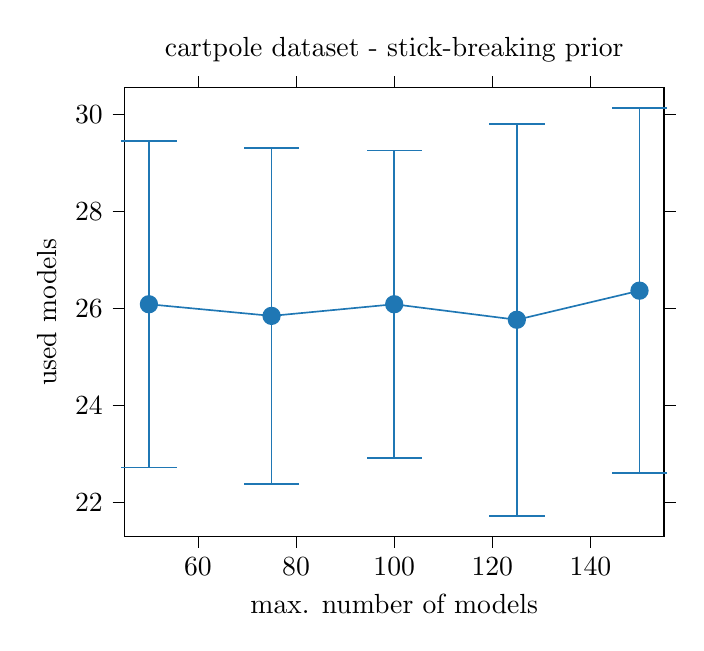
\begin{tikzpicture}

\definecolor{color0}{rgb}{0.12156862745098,0.466666666666667,0.705882352941177}

\begin{axis}[
tick align=outside,
tick pos=both,
title={cartpole dataset - stick-breaking prior },
x grid style={white!69.01960784313725!black},
xlabel={max. number of models},
xmin=45, xmax=155,
xtick style={color=black},
y grid style={white!69.01960784313725!black},
ylabel={used models},
ymin=21.2972128031827, ymax=30.5419155015809,
ytick style={color=black}
]
\path [draw=color0, semithick]
(axis cs:50,22.7104896498156)
--(axis cs:50,29.4495103501844);

\path [draw=color0, semithick]
(axis cs:75,22.3795953993789)
--(axis cs:75,29.3004046006211);

\path [draw=color0, semithick]
(axis cs:100,22.9061064920196)
--(axis cs:100,29.2538935079804);

\path [draw=color0, semithick]
(axis cs:125,21.7174265622008)
--(axis cs:125,29.8025734377992);

\path [draw=color0, semithick]
(axis cs:150,22.5982982574372)
--(axis cs:150,30.1217017425628);

\addplot [semithick, color0, mark=-, mark size=10, mark options={solid}, only marks]
table {%
50 22.7104896498156
75 22.3795953993789
100 22.9061064920196
125 21.7174265622008
150 22.5982982574372
};
\addplot [semithick, color0, mark=-, mark size=10, mark options={solid}, only marks]
table {%
50 29.4495103501844
75 29.3004046006211
100 29.2538935079804
125 29.8025734377992
150 30.1217017425628
};
\addplot [semithick, color0, mark=*, mark size=3, mark options={solid}]
table {%
50 26.08
75 25.84
100 26.08
125 25.76
150 26.36
};
\end{axis}

\end{tikzpicture}
